\documentclass{article}

\usepackage{afterpage}
\usepackage{fontspec}
\usepackage{geometry}
\usepackage{hyperref}
\usepackage{lscape}
\usepackage{pgfgantt}
\usepackage{siunitx}
\usepackage{titling}

\title{CRAPS Kernel}
\author{
       Maxime Arthaud
  \and Korantin Auguste
  \and Martin Carton
  \and Étienne Lebrun
  \and Pierre-Louis Michel
}

\begin{document}
  \begin{titlepage}
  \begin{center}
    
\includegraphics[height=1cm]{LogoEnseeiht}\\\vspace{1cm}
    \hrule\vspace{0.5cm}
    \textsc{\Large\thesubtitle}
    \\\vspace{0.5cm}

    \textbf{\huge\thetitle}
    \\\vspace{0.4cm}
    \hrule\vspace{2cm}

    {\large
      Maxime~\textsc{Arthaud}      \\
      Korantin~\textsc{Auguste}    \\
      Martin~\textsc{Carton}       \\
      Étienne~\textsc{Lebrun}
    }

    \vfill
    {\large January -- March 2015}
  \end{center}
\end{titlepage}

  \tableofcontents
  \newpage

  \section{Introduction}
    This project, suggested by Daniel Hagimont, is based on the CRAPS processor
    developed by Jean-Christophe Buisson and used in the first-year CPU
    architecture courses at ENSEEIHT. The goal is to develop an operating
    system that would run on top of that processor.

    The reasons for that project are that before, it was only possible to do a
    little of assembly directly on the processor to see it work, but nothing
    more.  After our project, it should be possible for students to really see
    the layer that goes on top of the CPU in modern computers: the operating
    system. So that the students can really make the link between the processor
    they just built and the computer and underlying operating systems they use
    everyday.

    \paragraph{}
    The system will be as modular as possible, so that students can reuse parts
    of it and implement their own modules.

  \section{Project Overview}
    The objective of the project is to create an operating system, with a
    scheduler running a few tasks. It will also provide functions to display
    text to the user, do input/output to a permanent storage\dots

    For now, having the OS loading programs dynamically is out-of-scope : the
    goal is to have a very simple functional OS.  We will also have to improve
    the CPU to make it support our OS. Specifically we know we will have to
    support the RAM chips that are on the FPGA: currently, we have \SI{2}{kB}
    of RAM that are built in, but that's clearly not enough. Another important
    and time-consuming element will be to reuse the compiler we made last year
    during a project, and adapt it to generate the CRAPS assembly. We will
    surely need to make other modifications to the compiler.

  \section{Method, Tools and Test Means}
    Tests are quite a though point, as our only mean of real test is to put our
    code on the board and try it. That's why we want to proceed iteratively and
    start with very basic things.

    At the end, we want to be able to run a few processes that will communicate
    to the user, and store data in permanent memory.

  \section{Software Team Organisation and Responsibilities}
    \begin{itemize}
      \item Martin Carton as \textit{project leader}
      \item Korantin Auguste
      \item Maxime Arthaud
      \item Étienne Lebrun
      \item Pierre-Louis Michel
    \end{itemize}

  \section{Project Monitoring and Controls}
    A Gantt diagram for the project is available on page \pageref{fig:gantt}.

    Controls: meetings?

    \afterpage{\newgeometry{top=2cm,bottom=3.5cm}
\begin{landscape}
  \label{fig:gantt}
  \def\pgfcalendarweekdayletter#1{%
    \ifcase#1M\or T\or W\or T\or F\or S\or S\fi%
  }
  \thispagestyle{empty}
  \centering
  \noindent\resizebox{\linewidth}{!}{
    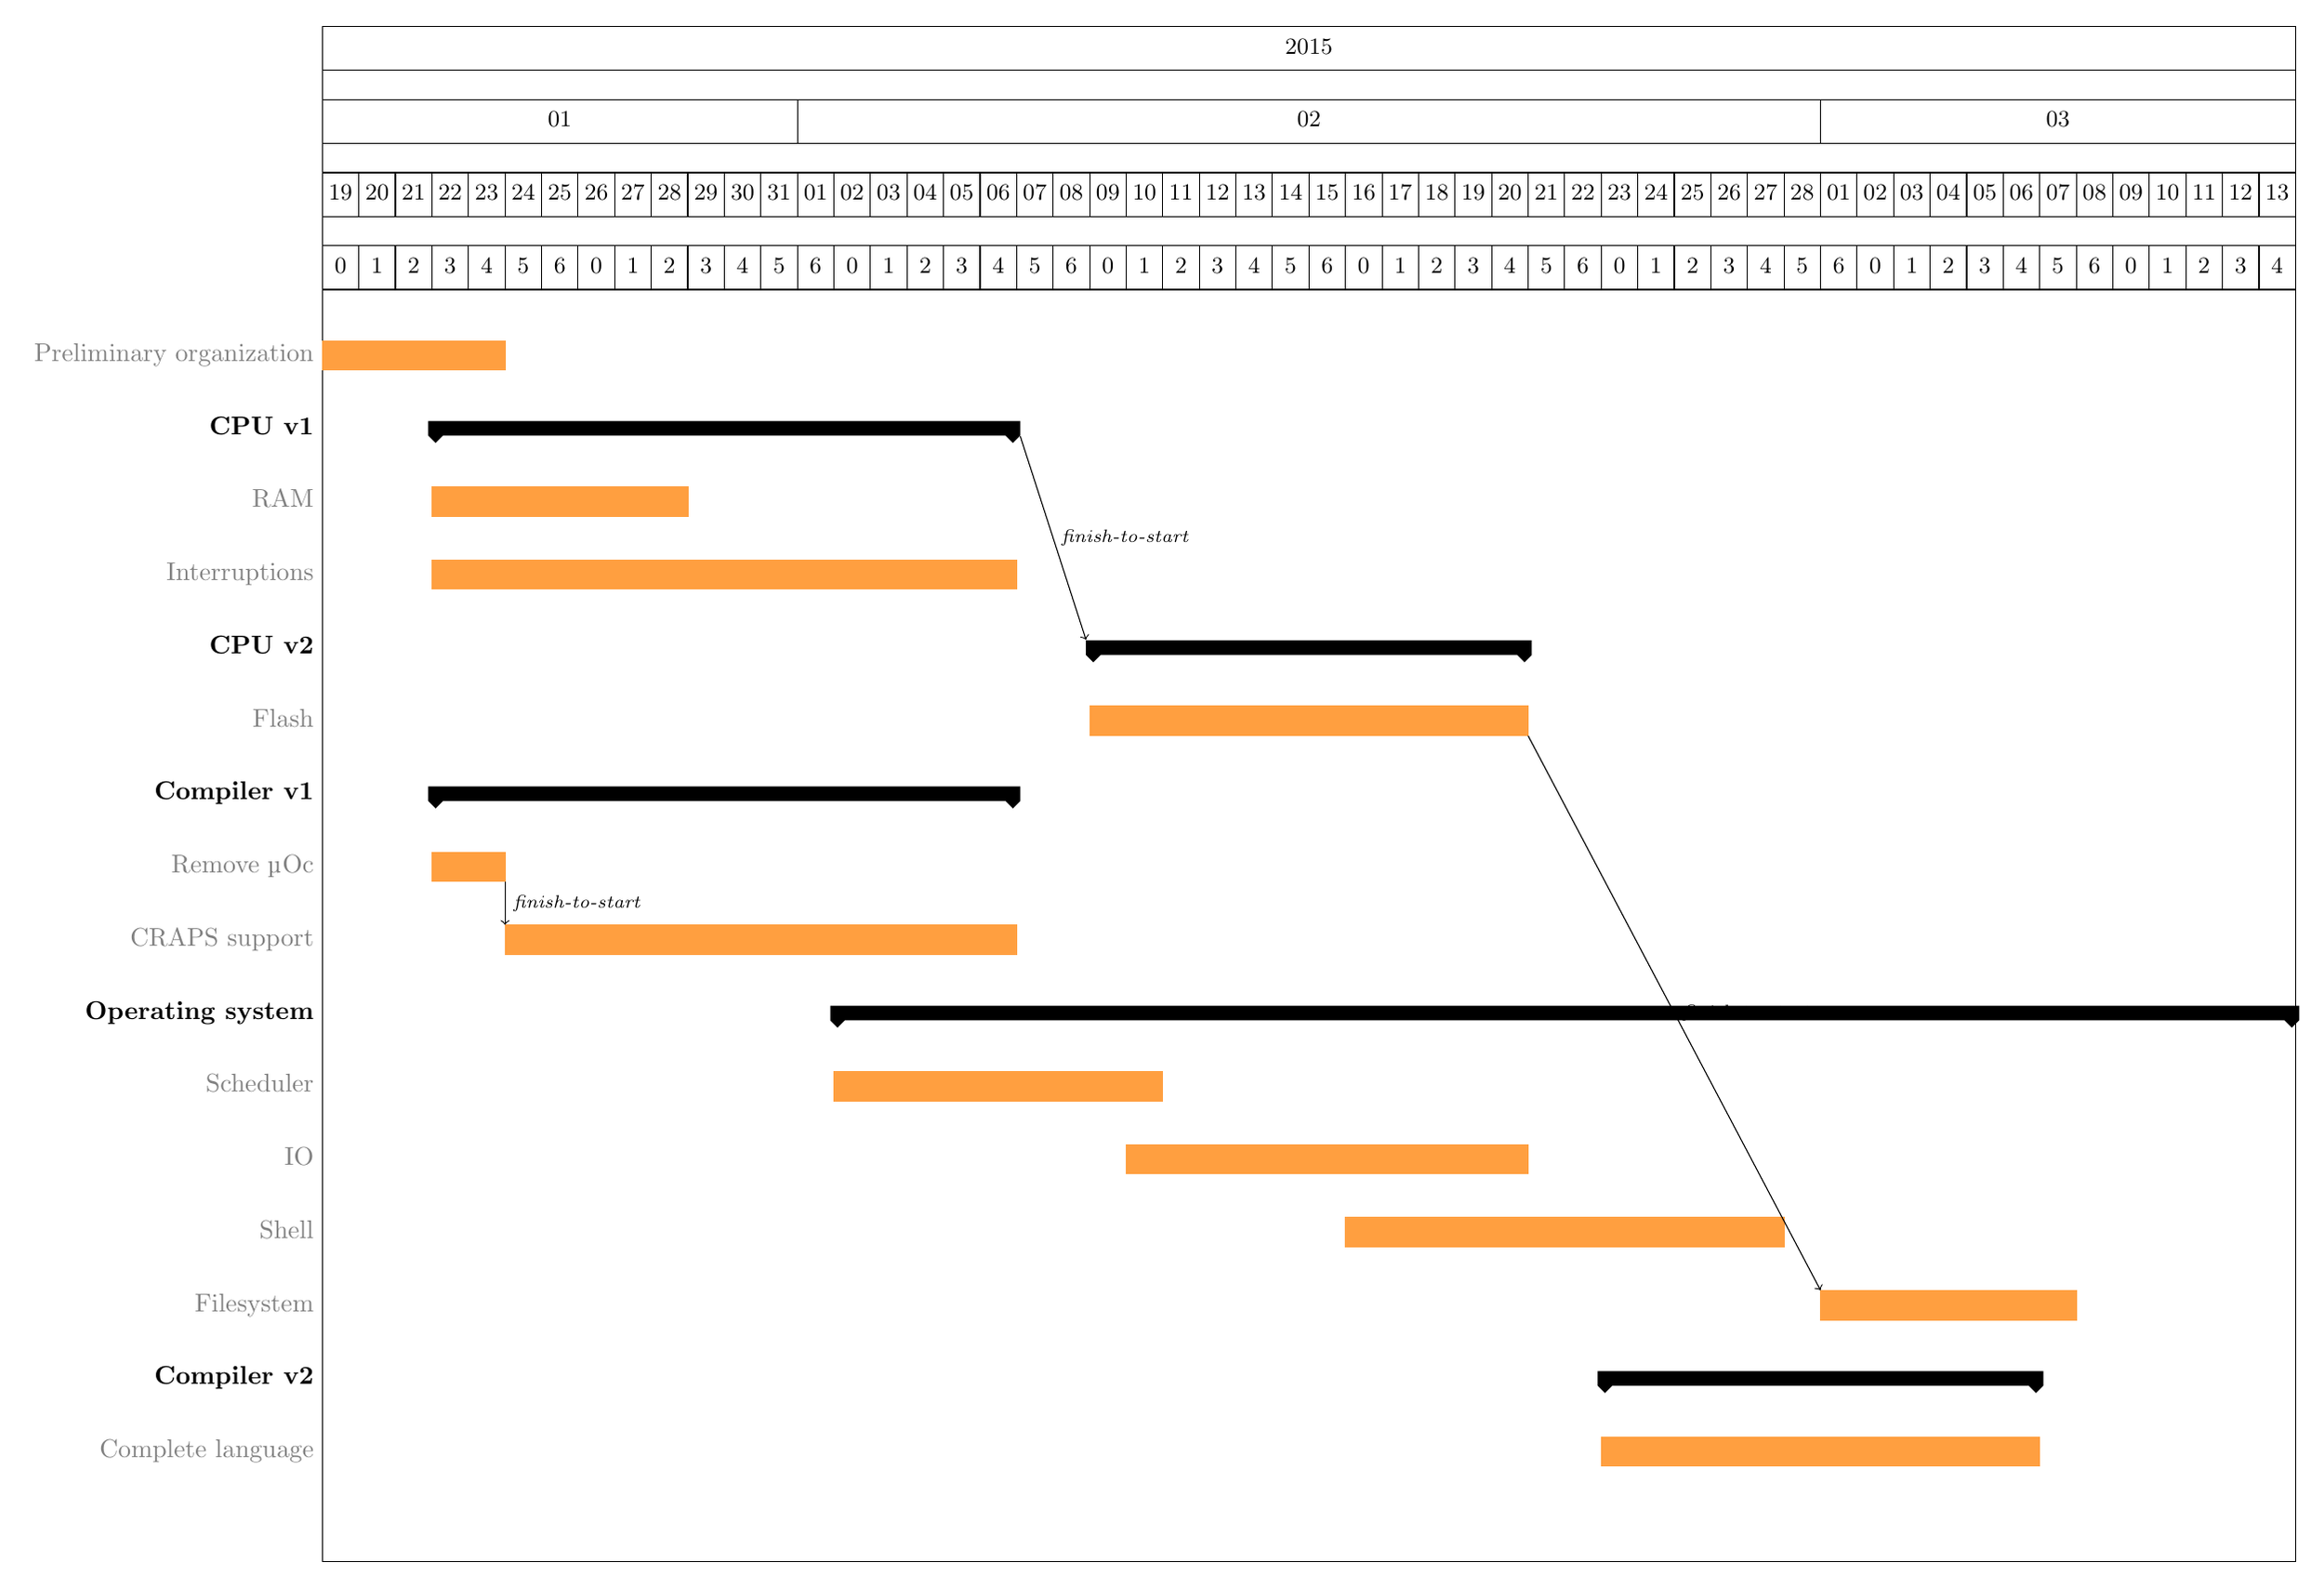
\begin{tikzpicture}
      \begin{ganttchart}[
          /pgf/outer xsep=+0pt,
          bar/.append style={orange!75},
          time slot format=isodate,
          link/.style={->},
          bar label font=\normalsize\color{black!50}
        ]{2015-01-19}{2015-03-13}
        \gantttitlecalendar{year, month, day, weekday=letter}                 \\

        \ganttbar{Preliminary organization}{2015-01-19}{2015-01-23}           \\

        \ganttgroup[name=CPU1]{CPU v1}{2015-01-22}{2015-02-06}                \\
            \ganttbar[name=RAM]{RAM}{2015-01-22}{2015-01-28}                  \\
            \ganttbar[name=IT]{Interruptions}{2015-01-22}{2015-02-06}         \\

        \ganttgroup[name=CPU2]{CPU v2}{2015-02-09}{2015-02-20}                \\
            \ganttlink[link type=f-s]{CPU1}{CPU2}
            \ganttbar[name=flash]{Flash}{2015-02-09}{2015-02-20}              \\

        \ganttgroup[name=comp1]{Compiler v1}{2015-01-22}{2015-02-06}          \\
            \ganttbar[name=MOC]{Remove µOc}{2015-01-22}{2015-01-23}           \\
            \ganttbar[name=CRAPS]{CRAPS support}{2015-01-24}{2015-02-06}      \\

        \ganttgroup[name=os]{Operating system}{2015-02-02}{2015-03-13}        \\
            \ganttbar{Scheduler}{2015-02-02}{2015-02-10}                      \\
            \ganttbar{IO}{2015-02-10}{2015-02-20}                             \\
            \ganttbar{Shell}{2015-02-16}{2015-02-27}                          \\
            \ganttbar[name=FS]{Filesystem}{2015-02-29}{2015-03-07}            \\

            \ganttlink[link type=f-s]{flash}{FS}

        \ganttgroup[name=comp2]{Compiler v2}{2015-02-23}{2015-03-06}          \\
            \ganttbar[name=MOREC]{Complete language}{2015-02-23}{2015-03-06}  \\

            \ganttlink[link type=f-s]{MOC}{CRAPS}
      \end{ganttchart}
    \end{tikzpicture}
  }
\end{landscape}
\restoregeometry
}

  \section{Meetings and reporting}
    A meeting with the client will be planned once a week. A meeting with the
    industrial supervisor is also planned once a week.

  \section{Management of actions}
    A file with the actions (who did what and when as be created).

  \section{Management of risks}
    \begin{itemize}
      \item A FPGA can be damaged, making any test impossible. This is likely to
          happen but we have two FPGA and the possibility to have more in case
          of problem.
      \item We may not be able to integrate the RAM, leading to huge memory
          limitations that may make the project impossible
    \end{itemize}

  \section{Management of change requests}

  \section{Quality and Configuration management}
    Use of a version control system: a Git repository on Github.

  \section{Documentation}
    As the system will be modular and expected to be used by students, a
    documentation of every module will be provided.

    \begin{itemize}
      \item User Manual
      \item modified CRAPS
    \end{itemize}

  \newpage
  \begin{appendix}
    \section{Specifications}
      \begin{itemize}
        \item Improvement of the processor
          \begin{itemize}
            \item support of the RAM chip on the FPGA to have more than
              \SI{2}{kB} of memory.
            \item support of the I/O we need for the permanent storage
            \item support of a serial port or any other peripheral to
              communicate with the user
          \end{itemize}
        \item Compiler
          \begin{itemize}
            \item CRAPS assembly backend
            \item make the source language as much similar as C
          \end{itemize}
          \item Development of the OS
            \begin{itemize}
              \item test task 1: make a led blink
              \item test task 2: communicate with the user
                \begin{itemize}
                  \item development of a mini-shell ?
                  \item management of the I/O from the software
                \end{itemize}
              \item scheduler and process management
              \item system calls and API of the OS:
                \begin{itemize}
                  \item very simple file system
                  \item user I/O (using the serial port or other means)
                  \item system task to manage the I/O?
                  \item functions like \verb+malloc+, etc.
                \end{itemize}
            \end{itemize}
        \item Report
          \begin{itemize}
            \item write the developer documentation
          \end{itemize}
      \end{itemize}
  \end{appendix}
\end{document}
